%!TEX root = ../main.tex

\subsection*{Ejercicio 5.}
\begin{enumerate}
    \item[(a)] Simplifique el algoritmo de eliminación de Gauss para resolver un sistema lineal $Ax = b$ donde $A$ es una matriz tridiagonal.

    $$
A=\left(\begin{array}{ccccc}
a_{11} & a_{12} & & & \\
a_{12} & a_{22} & a_{23} & & \\
& \ddots & \ddots & \ddots & \\
& & a_{n-1, n-1} & a_{n-1, n-1} & a_{n-1, n} \\
& & & a_{n-1, n} & a_{n, n}
\end{array}\right) \in \mathbb{R}^{n \times n}
$$

    \begin{solution}
        La idea del algoritmo simplificado es que al realizar eliminación de Gauss no es necesario calcular los elementos debajo de la diagonal, además en cada iteración del método, solo nos quedan dos elementos no nulos por cada fila, el elemento en la diagonal $a_{i,i}$ y $a_{i,i+1}$, por lo tanto en la siguiente iteración solo debemos calcular el cambio realizado al elemento $a_{i+1,i+1}$, a saber, el siguiente en la diagonal, ya que el otro término se vuelve cero.\\

        Para dejarlo más claro presentaremos el algoritmo, teniendo en cuenta que debemos aplicar el método también al vector $b$.

\textbf{1. Eliminación Gaussiana}

\begin{itemize}
    \item \textbf{Para} $i = 2,\ldots,n$:
    \begin{itemize}
        \item Calcular el multiplicador: 
        \[
        m = \frac{a_{i-1, i}}{a_{i-1, i-1}}
        \]
        \item Actualizar la diagonal principal:
        \[
        a_{i, i} \leftarrow a_{i, i} - m \cdot a_{i-1, i}
        \]
        \item Actualizar el vertor $b$:
        \[
        b_i \leftarrow b_i - m \cdot b_{i-1}
        \]
    \end{itemize}
\end{itemize}

\textbf{2. Sustitución hacia atrás:} Como la matriz solo tiene dos entradas por fila, el algoritmo se reduce a 

\begin{itemize}
    \item Inicio:
    \[
    x_n = \frac{b_n}{a_{n, n}}
    \]
    \item \textbf{Para} $i = n-1$ \textbf{hasta} $1$:
    \begin{itemize}
        \item Calcular:
        \[
        x_i = \frac{b_i - a_{i, i+1} \cdot x_{i+1}}{a_{i, i}}
        \]
    \end{itemize}
\end{itemize}

\textbf{3. Retornamos:}
\[
x = (x_1, x_2, \dots, x_n)
\]

    \end{solution}
    \item[(b)] Considere la ecuación de Poisson con término fuente $f$ en el intervalo $(0, 1)$:
    \[
    -T''(x) = f(x), \quad x \in (0, 1),
    \]
    con condiciones de frontera $T(0) = T(1) = 0$. Aproximando la segunda derivada por diferencias finitas:
    \[
    T''(x) \approx \frac{T(x-h) - 2T(x) + T(x+h)}{h^2},
    \]
    y discretizando en $x_i = i h$, $i = 0, 1, \ldots, n$, con $n = 1/h$, obtenemos el sistema:
    \[
    -T_{i-1} + 2T_i - T_{i+1} = h^2 f(x_i), \quad i = 1, \ldots, n-1.
    \]
    Escriba este sistema en la forma $A T = f$, donde $A$ es una matriz tridiagonal. Resuelva el sistema para $n = 1000$ y $f(x) = \sin(2\pi x)$. Compare su solución con $T(x) = \sin(2\pi x) / (4\pi^2)$.
\end{enumerate}

\begin{solution}
    Primero escribimos el sistema de ecuaciones en forma matricial, obtenemos una matriz de tamaño $(n-1)\times (n-1)$, los términos $T_0 $ y $T_n$ los tratamos por aparte ya que son las condiciones de frontera. La solución numérica de la ecuación se obtiene de resolver el sistema

    $$
\left[\begin{array}{rrrrrr}
2 & -1 & 0 & 0 & \ldots & 0 \\
-1 & 2 & -1 & 0 & \ldots & 0 \\
0 & -1 & 2 & -1 & \ldots & 0 \\
\vdots & \ddots & \ddots & \ddots & \ddots & \vdots \\
0 & \ldots & 0 & -1 & 2 & -1 \\
0 & 0 & \ldots & 0 & -1 & 2
\end{array}\right]\left[\begin{array}{c}
T_1 \\
T_2 \\
T_3 \\
\vdots \\
T_{n-2} \\
T_{n-1}
\end{array}\right]=\left[\begin{array}{c}
h^2 f(h)\\
h^2 f(2h) \\
h^2 f(3h) \\
\vdots \\
h^2 f(nh-2h) \\
h^2 f(nh-h)
\end{array}\right],
$$

sabemos que la solución de la ecuación debe ser de clase $C^2_{\text{per}}([0,1])$ ya que $T(0)=T(1)$. Si $f(x)=\sin(2\pi x)$, podemos aplicar el algoritmo de eliminación de Gauss que hemos simplificado para matrices tridiagonales en el paso anterior.\\

Implementamos el algoritmo en python y comparamos con la solución exacta $T(x)=\sin(2\pi x)/(4\pi^2)$ usando matplotlib, obtuvimos

\begin{center}
    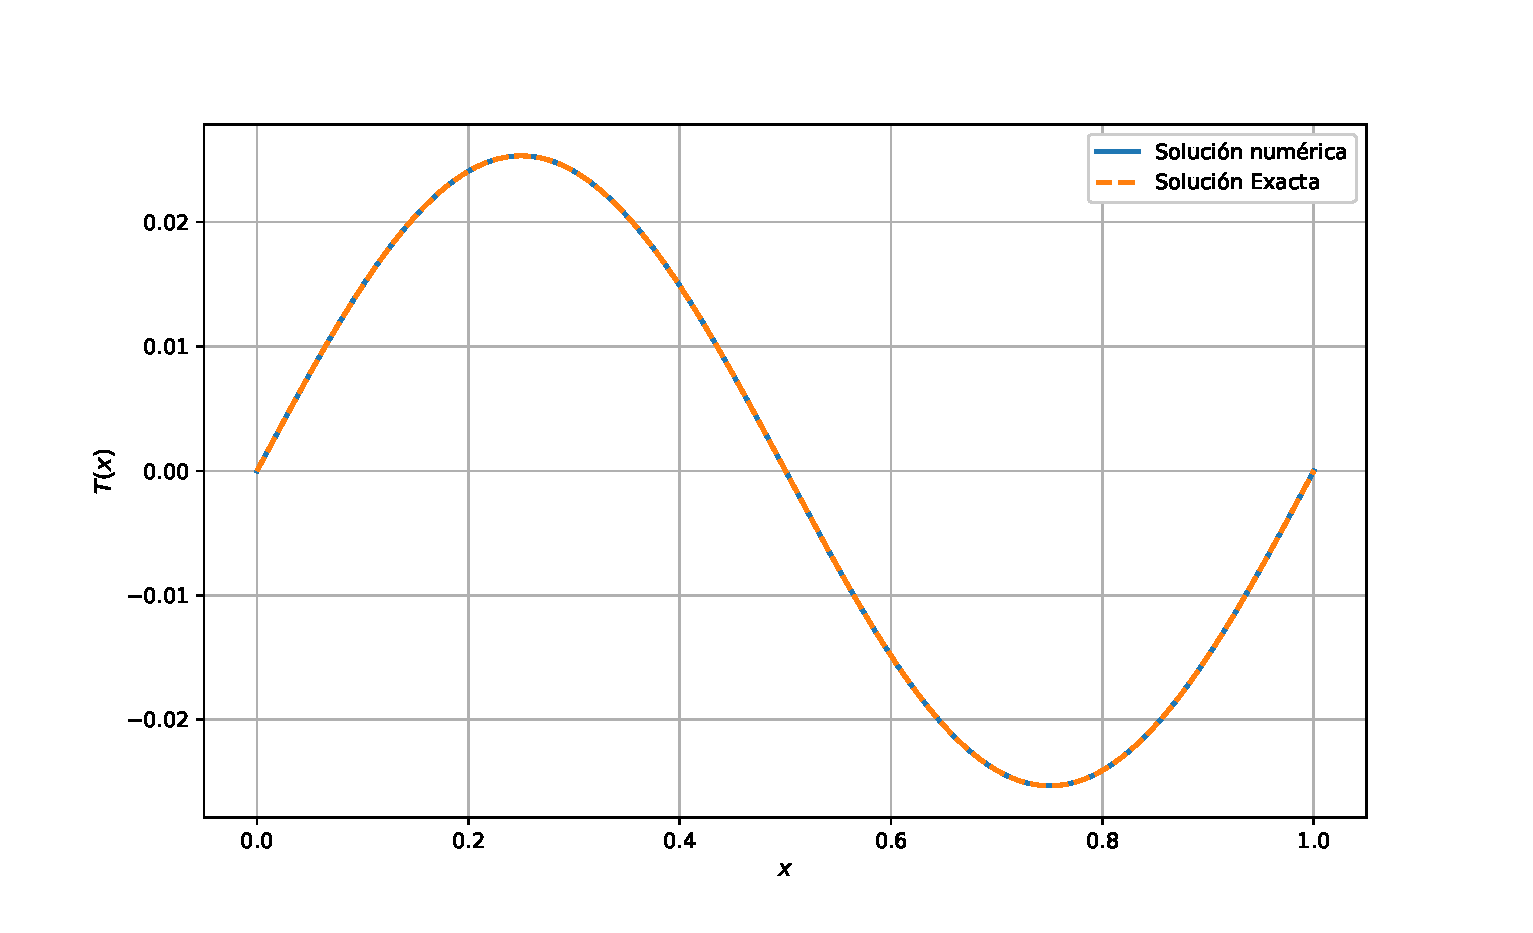
\includegraphics[scale=0.6]{Nucoyoyoyoyoyoyoyo.eps}
\end{center}

También obtuvimos el error máximo, $8.333350\times 10^{-8}$, lo que nos dice que la solución es buena tomando como tamaño del paso $h=1/1000$ en las diferencias finitas.

\end{solution}